\chapter{Introduction}\label{1}

This chapter discusses the motivation, specific context, research gaps of literature, goals and research questions, overall methodological approach, and the list of scientific contributions.

\section{Background and Motivation}\label{Background}

To combat climate change, the production of greenhouse gas emissions must be reduced to significant levels and shift to use of \gls{RES} must be accomplished. In numbers, the European Union's (\gls{EU}) Nationally Determined Contribution (NDC) under the Paris Agreement is to reduce greenhouse gas emissions by at least 40\% by 2030 compared to 1990 \cite{agreement2015unfccc}. 

The plans involve a future target of nearly 70 GW to 150 GW offshore wind power in the North Sea by 2040. A scope of 140 to 450 GW of offshore wind power in the \gls{EU} by 2050 is seen from the latest European Commission situations. Nearly 13 GW of offshore wind capacity was installed in 2018 in the North Sea. Going with the current pace, the rate of offshore wind deployment is deficient in reaching the objectives of the Paris Agreement. To comply with these objectives, an extraordinary jump in offshore wind energy is required, as shown in Figure \ref{fig:Paris_roll_out}. An effective solution calls for an increase in large scale offshore wind deployment in the North Sea \cite{noauthor_vision_nodate}. As mentioned in \cite{noauthor_tennet_2020}, the Transmission System Operator (TSO) of the Netherlands, TenneT, has already entered into an innovation partnership with its suppliers to establish a 2 GW offshore platform to bring in their contribution towards the Paris Agreement. While the requirement for large scale networks is appealing, the technical challenges that could be encountered should also be considered.  

\begin{figure}[H]
\centering
%\hspace*{-1.2cm}
    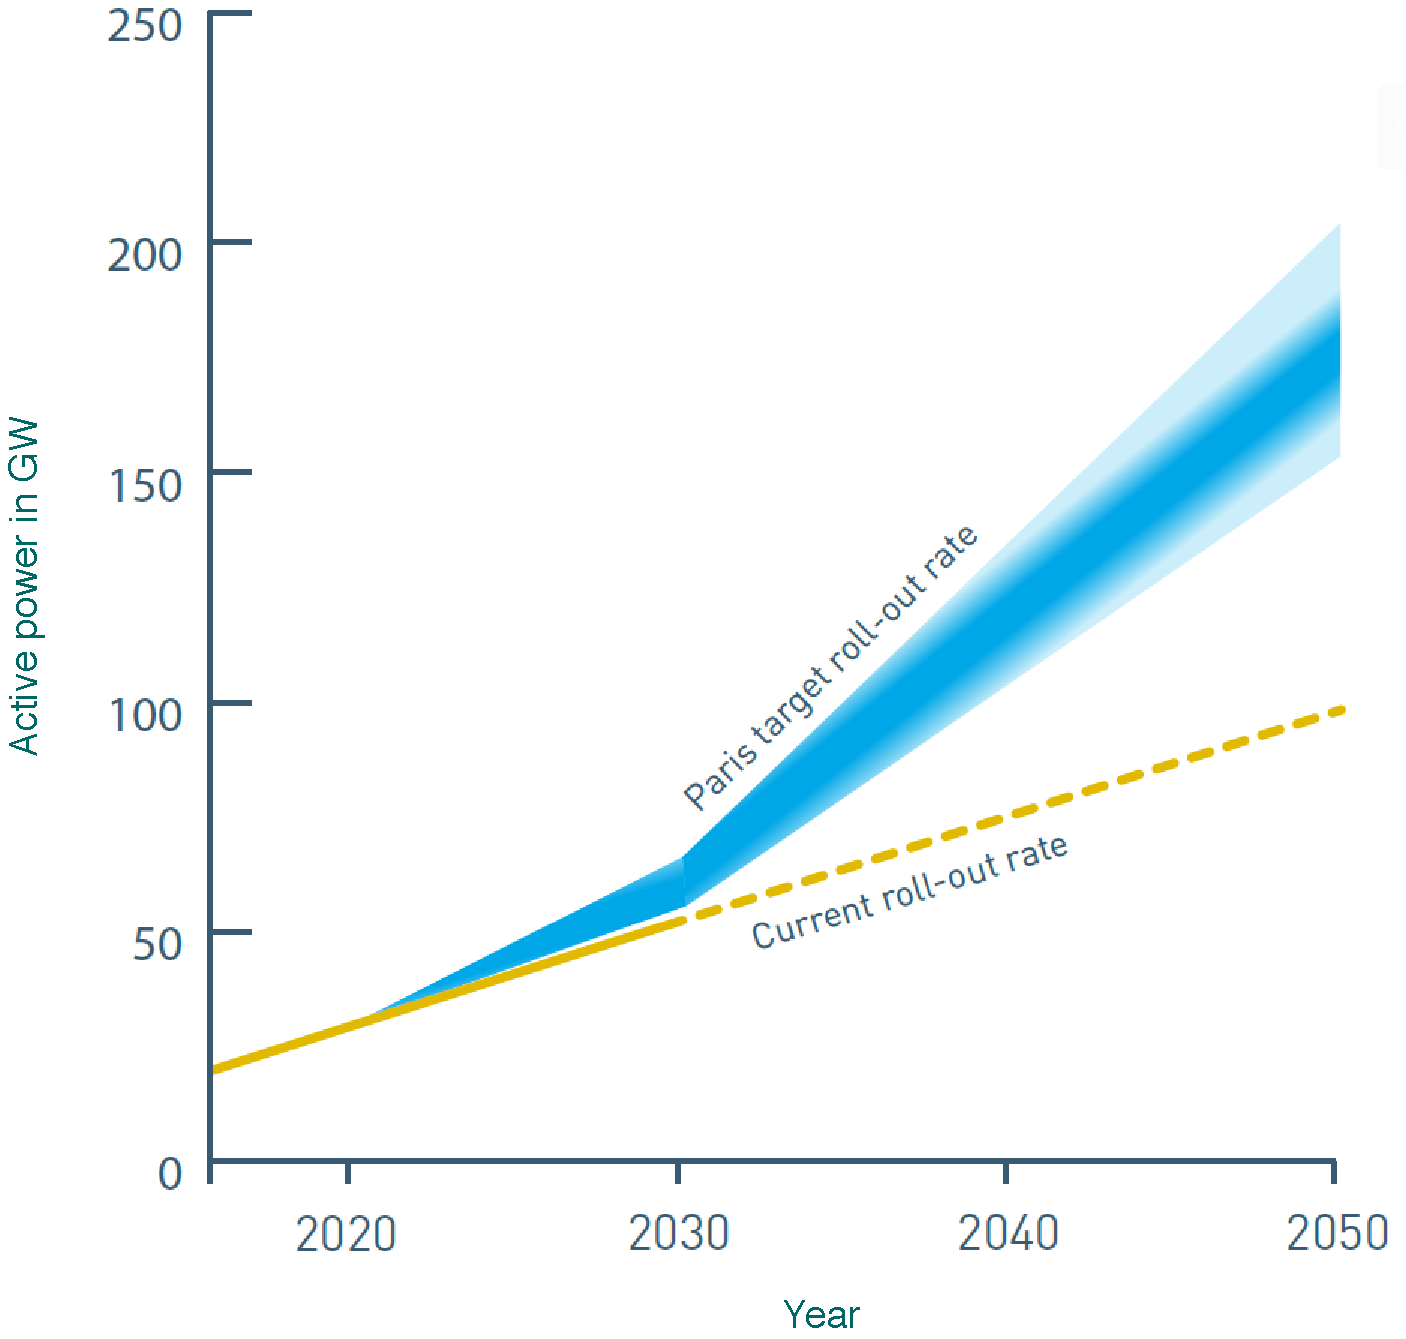
\includegraphics[height = 6.5cm,width = 7cm]{Diagrams/Chapter_1/Paris.pdf}
    \caption{Installed wind capacity in the North Sea in GW \cite{noauthor_vision_nodate}}
    \label{fig:Paris_roll_out}
\end{figure}

\gls{RES} are connected to the power system through Power Electronic (\gls{PE}) converters as shown in Figure \ref{fig:Energy_conv_system_2}. The \gls{PE} converters do not posses inherent inertial response characteristics. Until now integration of \gls{RES} has not created major problems since the stability of the system is maintained by the synchronous machines in power plants. Traditionally, the inertia for the power system is provided by these conventional units connected to the network (Figure \ref{fig:Energy_conv_system}). However, an increase in \gls{RES} in the future causes an increase in \gls{PE} converter based generation units. Simultaneously, conventional power plants using non-renewable energy sources need to be disconnected from the network. This makes the power systems weak due to low short circuit power available and low system inertia. The disconnection of conventional generators also requires the \gls{RES} connected through \gls{PE} converter based generation units to take up the role of governing the stability of the system.

\begin{figure}[H]
\centering
%\hspace*{-1.2cm}
    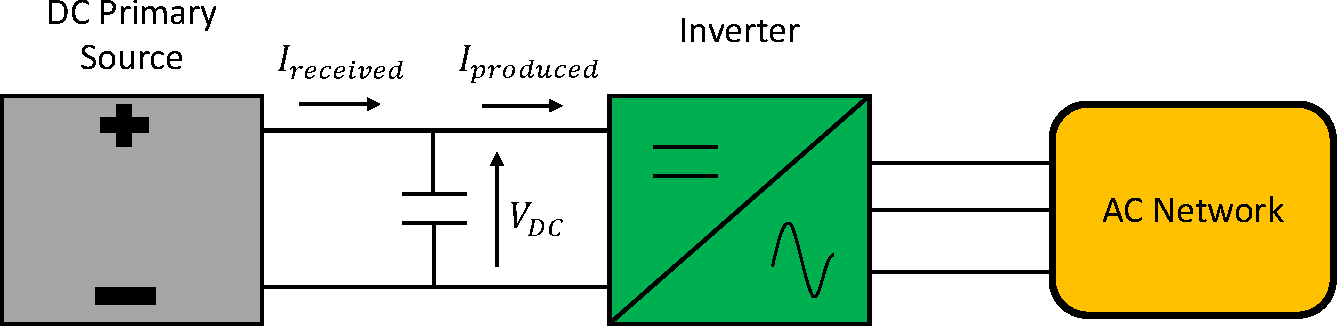
\includegraphics[height = 3cm,width = 12cm]{Diagrams/Chapter_1/Energy_conv_system_2.pdf}
    \caption{PE converter-based generation connection to the grid \cite{denis_migrate_2018}}
    \label{fig:Energy_conv_system_2}
\end{figure}
\vspace{0mm}
\begin{figure}[H]
\centering
%\hspace*{-1.2cm}
    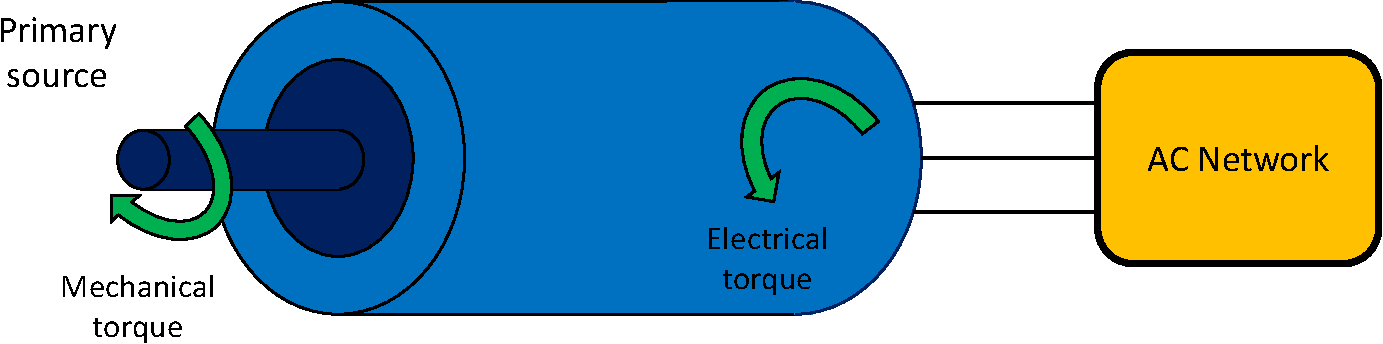
\includegraphics[height = 3cm,width = 12.5cm]{Diagrams/Chapter_1/Energy_conv_system.pdf}
    \caption{Conventional generators connection to the grid \cite{denis_migrate_2018}}
    \label{fig:Energy_conv_system}
\end{figure}

The majorly contributing source among the \gls{RES} is wind energy and the deployment of wind energy technology is expected to grow further. As the share of wind energy among the \gls{RES} increases, the integration of \gls{PE} converter based generation units becomes more challenging. The continuous variations in wind speed causes constant change in the active power output of the wind power plant. This could lead to an increase in the reactive power output and consequently voltage at the point of common coupling (\gls{PCC}). 

The conventional current control methods using Proportional Integral (\gls{PI}) controllers in the modern wind turbines are capable of providing voltage control by injecting reactive currents when connected to a strong network \footnote{SCR = SC$_{MVA}$/P;\; where SC$_{MVA}$ is the short circuit power of the network and P is the active power generation. \\
If SCR = 100 to 250, it is a strong grid. If SCR = 5 to 25, it is a weak grid.}, capable of absorbing the injected currents. However, these controllers are not suitable for operation in highly \gls{PE} converter dominated grids as the connected network is weak and is not capable of absorbing the injected currents. Furthermore, during the scenario of islanding, voltage control by the conventional controllers is ineffective as the deviation in voltage is not high enough to activate a productive voltage reduction mechanism. Moreover, the frequency of such an islanded network is not controlled as the conventional controllers in the wind generators are not equipped with such capability.  

       

Furthermore, the compelling need to move towards large scale offshore networks increases the challenges from the technical point of view.


The first significant challenge is the control of voltage and frequency by the \gls{PE} converters without the presence of conventional units in the grid. The absence of conventional generators would mean that the \gls{PE} converters will have to take into account the decreasing inertia of the system that leads to a faster dynamic behaviour and needs controllers with faster time response. 

The second major concern is with the Proportional Integral (\gls{PI}) based conventional current control methods available for the \gls{PE} converters. Currently, they are the most commonly used controllers due to the ease of operation. They are suitable for operation when connected to a strong network \footnote{SCR = SC$_{MVA}$/P;\; where SC$_{MVA}$ is the short circuit power of the network and P is the active power generation. \\
If SCR = 100 to 250, it is a strong grid. If SCR = 5 to 25, it is a weak grid.}. However, if overlooked, interactions among \gls{PI} controllers can persist in the grid with high \gls{PE} penetration and could lead to instability of the network.

The third critical challenge is the grid restoration following disturbances by the \gls{PE} converter units. With the conventional current control approach, grid restoration is challenging without the help of auxiliary diesel generators. However, in the case of increasing \gls{PE} converters, the role of grid restoration must be taken up by these converters. There can be arguments that storage facilities such as battery and thermal can be a realizable solution in case when there are no conventional generators available. Huge investment costs, low lifetime and low efficiency are the drawbacks when compared to controller modifications that make these storage facilities practically unusable in large scale power system \cite{telaretti_economic_2016}.  

Lastly, the connection of distant Offshore Wind Farms (\gls{OWF}s) also creates challenges for the system operators. High Voltage Direct Current (\gls{HVDC}) transmission is preferred over High Voltage Alternating Current (\gls{HVAC}) for longer distances due to lower losses and lower investment costs \cite{ryndzionek_evolution_2020}. Conventionally, in an offshore wind farm network, the offshore converter works in voltage control, and the wind turbine converters work in current control scheme. This could cause problems to the \gls{OWF} during severe dynamic scenarios. One such scenario is the reactive current injection that needs to be provided by the Wind Generators (\gls{WG}s) during dynamic conditions as demanded by majority of the grid codes \cite{mohseni_review_2012}. Therefore, the need for large scale offshore network and the technical challenges in integrating \gls{RES} to the grid has proved to be an important area of concern.

\section{Literature Review}

As seen in Section \ref{Background}, large scale deployment of \gls{OWF}s are a crucial requirement to meet the mentioned targets. So far, for small-sized wind farms, the offshore collector platform that connects all the \gls{WG}s and transfers power to the offshore converter station, has only contributed to a small part of the total expenditure. The reason being, the \gls{OWF}s mostly have radial collectors. This would not be the case when going for large scale wind farms. The critical area of concern will be the additional costs of subsea cables that require higher ratings and excess lengths \cite{quinonez-varela_electrical_2007}. The upcoming projects plan to have a higher rating of 66 kV compared to the conventional 33 kV \gls{HVAC} transmission due to the advantages of lesser array cabling, higher power transmission, a considerable decrease in capital expenditure and the avoidance of the \gls{AC} collector platform \cite{dnv66kv}. Different large scale topologies are being explored, and the conventional configurations are presented in \cite{guan_novel_2014}. However, the topology mentioned in \cite{lozada_ayala_dynamic_2018} embraces the utilization of 66 kV \gls{HVAC} transmission from the offshore \gls{AC} network directly to the offshore converter station. Such a topology could avoid the need for an offshore \gls{AC} collector platform and bring other benefits such as increased power transfer and reduced array cabling. The techno-economic assessment of such a configuration is depicted in \cite{misyris2020north}. 

Various control concepts are being explored to mitigate the technical challenges mentioned in the previous section due to the integration of \gls{RES}. Typically, \gls{RES} are connected to the grid for parallel operation using present state of the art technology, i.e. grid following control strategies, in which the regulation of power output of the converters is achieved by measuring the angle of the grid voltage. The drawback of these controllers is that they require an already existing grid voltage. However, the V/F (voltage/frequency) control mode is used for operation in the islanded mode where the voltage is created by the V/F control. The issue concerned with this control is that it is not equipped for the parallel operation of various voltage forming units \cite{weise2019comparison}. New control strategies that can create the grid voltage and work in parallel operation is an emerging area of research. ENTSO-E classifies converters into three classes (Class 1, Class 2 and Class 3) and the converters working with the strategies mentioned above are categorized under Class 3. The complete requirements that need to be complied by such converters are depicted in \cite{christensen2020high}.

The new control strategies available for grid parallel and island operation are as follows:
\begin{itemize}
    \item Virtual Synchronous Machines (VSM): The characteristic of synchronous machines in terms of inertia and voltage support is imitated by correspondingly deriving the equations for control \cite{chen_comparison_2012}, \cite{duckwitz_operating_behavior}, \cite{lu_virtual_2019}.
    
    \item Modified Droop Control:
    For decentralized grids, the parallel operation of voltage forming units is developed recently using the f/P (frequency/active power) and V/Q (voltage/reactive power) droop controls similar to the control in synchronous generators \cite{lopes2012pv}. Few authors have named these droop control concepts as Virtual Synchronous Machines Without Inertia (VSCM0H) \cite{yu2016use}.
    
    \item Direct Voltage Control (\gls{DVC}):
    The \gls{DVC} control allows for the direct control of the \gls{AC} converter voltage which in turn varies the current injected by the converter  \cite{korai_dynamic_2019}, \cite{erlich_new_2017}. This approach provides continuous control both in steady-state and dynamic scenarios. This control method is implemented for analysis in this thesis work.
    
    \item Extended Current Control:
    The control is similar to the classical current control with an additional inertia control in the outer control loop by using a df/dt controller that gives a behaviour similar to that of a synchronous machine \cite{duckwitz_derivation_2019}. 
    
\end{itemize}



\section{Objectives and Research Questions}
The overall goal of the thesis is to implement an enhanced control strategy for wind turbine generators in Voltage Source Converter - High Voltage Direct Current (\gls{VSC}-\gls{HVDC}) systems in \gls{EMT} simulators and to perform analysis on the dynamics of voltage and power flows within a large scale offshore transmission network. Electro-Magnetic Transient (\gls{EMT}) simulation-based software tools are utilized in this thesis to analyze the performance of the developed control models. The thesis makes use of the average model of Type-4 \gls{WG} available in RSCAD as the basis. The \gls{EMT} based simulation interface in DIgSILENT PowerFactory tool is utilized as well. This report provides a detailed description of the different available features in RSCAD that are employed to develop a large scale model. 
To achieve the overall goal, the following research questions are defined:
\begin{itemize}
    \item How effective is the Direct Voltage Control (\gls{DVC}) when implemented in an \gls{EMT} average model of Type-4 \gls{WG} connected to a 66 kV equivalent \gls{HVAC} system in RSCAD?
    
    \item What insights can be attained by the \gls{EMT} average model of Type-4 \gls{WG} with \gls{DVC} in 66 kV network in RSCAD in comparison with a similar system modelled with a simplified Type-4 \gls{WG} configuration with \gls{DVC} in DIgSILENT PowerFactory?
    
    \item How can Type-4 \gls{WG}s with implemented \gls{DVC} work in coordination with offshore Modular Multi-level Converters (\gls{MMC}s) within a multi-gigawatt offshore transmission network?
    
    \item How effectively do Type-4 \gls{WG}s with implemented \gls{DVC} perform when connected in parallel operation?

\end{itemize}

\section{Thesis Contribution}
On behalf of the thesis objectives defined above, the methodology followed in this thesis is presented in this section.

\begin{itemize}
    \item Implementation of the \gls{DVC} in Type-4 \gls{WG} model in RSCAD for an offshore 66 kV \gls{HVAC} network. With proper documentation provided in this report, the developed 66 kV \gls{HVAC} model in RSCAD can be utilized for future work.
    
    \item Modelling of a 66 kV \gls{HVAC} network in PowerFactory by adapting the benchmark \gls{DVC} model in Type-4 \gls{WG}s. With proper documentation provided in this report, the developed 66 kV \gls{HVAC} mode in PowerFactory model can be utilized for future work.
    
    \item Development of a Multi-Gigawatt 66 kV offshore network model with \gls{DVC} implemented in Type-4 \gls{WG}s connected to a 2 GW offshore converter station in RSCAD. With proper documentation provided in this report, the developed 2 GW model in RSCAD can be utilized for future work.
    
    \item Automation script for the operation of the developed large scale offshore model using the interface between RSCAD and MATLAB is created. With
    proper documentation provided in this report, the script can be utilized for future work.
\end{itemize}

\section{Thesis Outline}
A brief outline of the main chapters is presented below, and a figurative representation of the thesis workflow is presented in Figure \ref{fig:Thesis_outline}.:
\begin{itemize}
    \item Chapter \ref{2}: The chapter presents the concepts of wind energy conversion system and the classification of wind turbines. The overview of the offshore wind farm system with all the major equipment and the latest trend in technology is explained. The issues with the present control structures and the necessity to move towards better control strategies are addressed. A new control structure implemented in this thesis is also formulated.  
    
    \item Chapter \ref{3}: The implementation of the identified control strategy in \cite{korai_dynamic_2019} and \cite{sethi_real-time_nodate-new} for a 66 kV \gls{HVAC} network model in RSCAD is detailed. The performance of Type-4 \gls{WG} with \gls{DVC}, in terms of reactive current injection, under severe disturbances is analyzed. Modelling of a similar 66 kV \gls{HVAC} network in DIgSILENT PowerFactory tool is also addressed. The comparison of the dynamic performance of the \gls{DVC} in two \gls{EMT} platforms (RSCAD and PowerFactory) for a 66 kV \gls{HVAC} offshore network during severe disturbances is carried out. 
    
    \item Chapter \ref{4}: The development of a large scale 2 GW offshore network model in RSCAD is detailed. The modifications in the control structures of the \gls{MMC}s to work in coordination with the implemented \gls{DVC} in \gls{WG}s are addressed.
    
    \item Chapter \ref{5}: The operation of the large scale network is discussed. The interplay of offshore \gls{MMC}s and Type-4 \gls{WG}s in terms of dynamic power flow control within the offshore network (by analyzing the voltage and current profiles in the electrical path between the \gls{WG}s and the \gls{MMC}s) is performed. 
    
    \item Chapter \ref{6}: The significant conclusions for the research questions are provided. The future scope and recommendations are also added.
\end{itemize}

\begin{figure}[H]
\centering
%\hspace*{-1.2cm}
    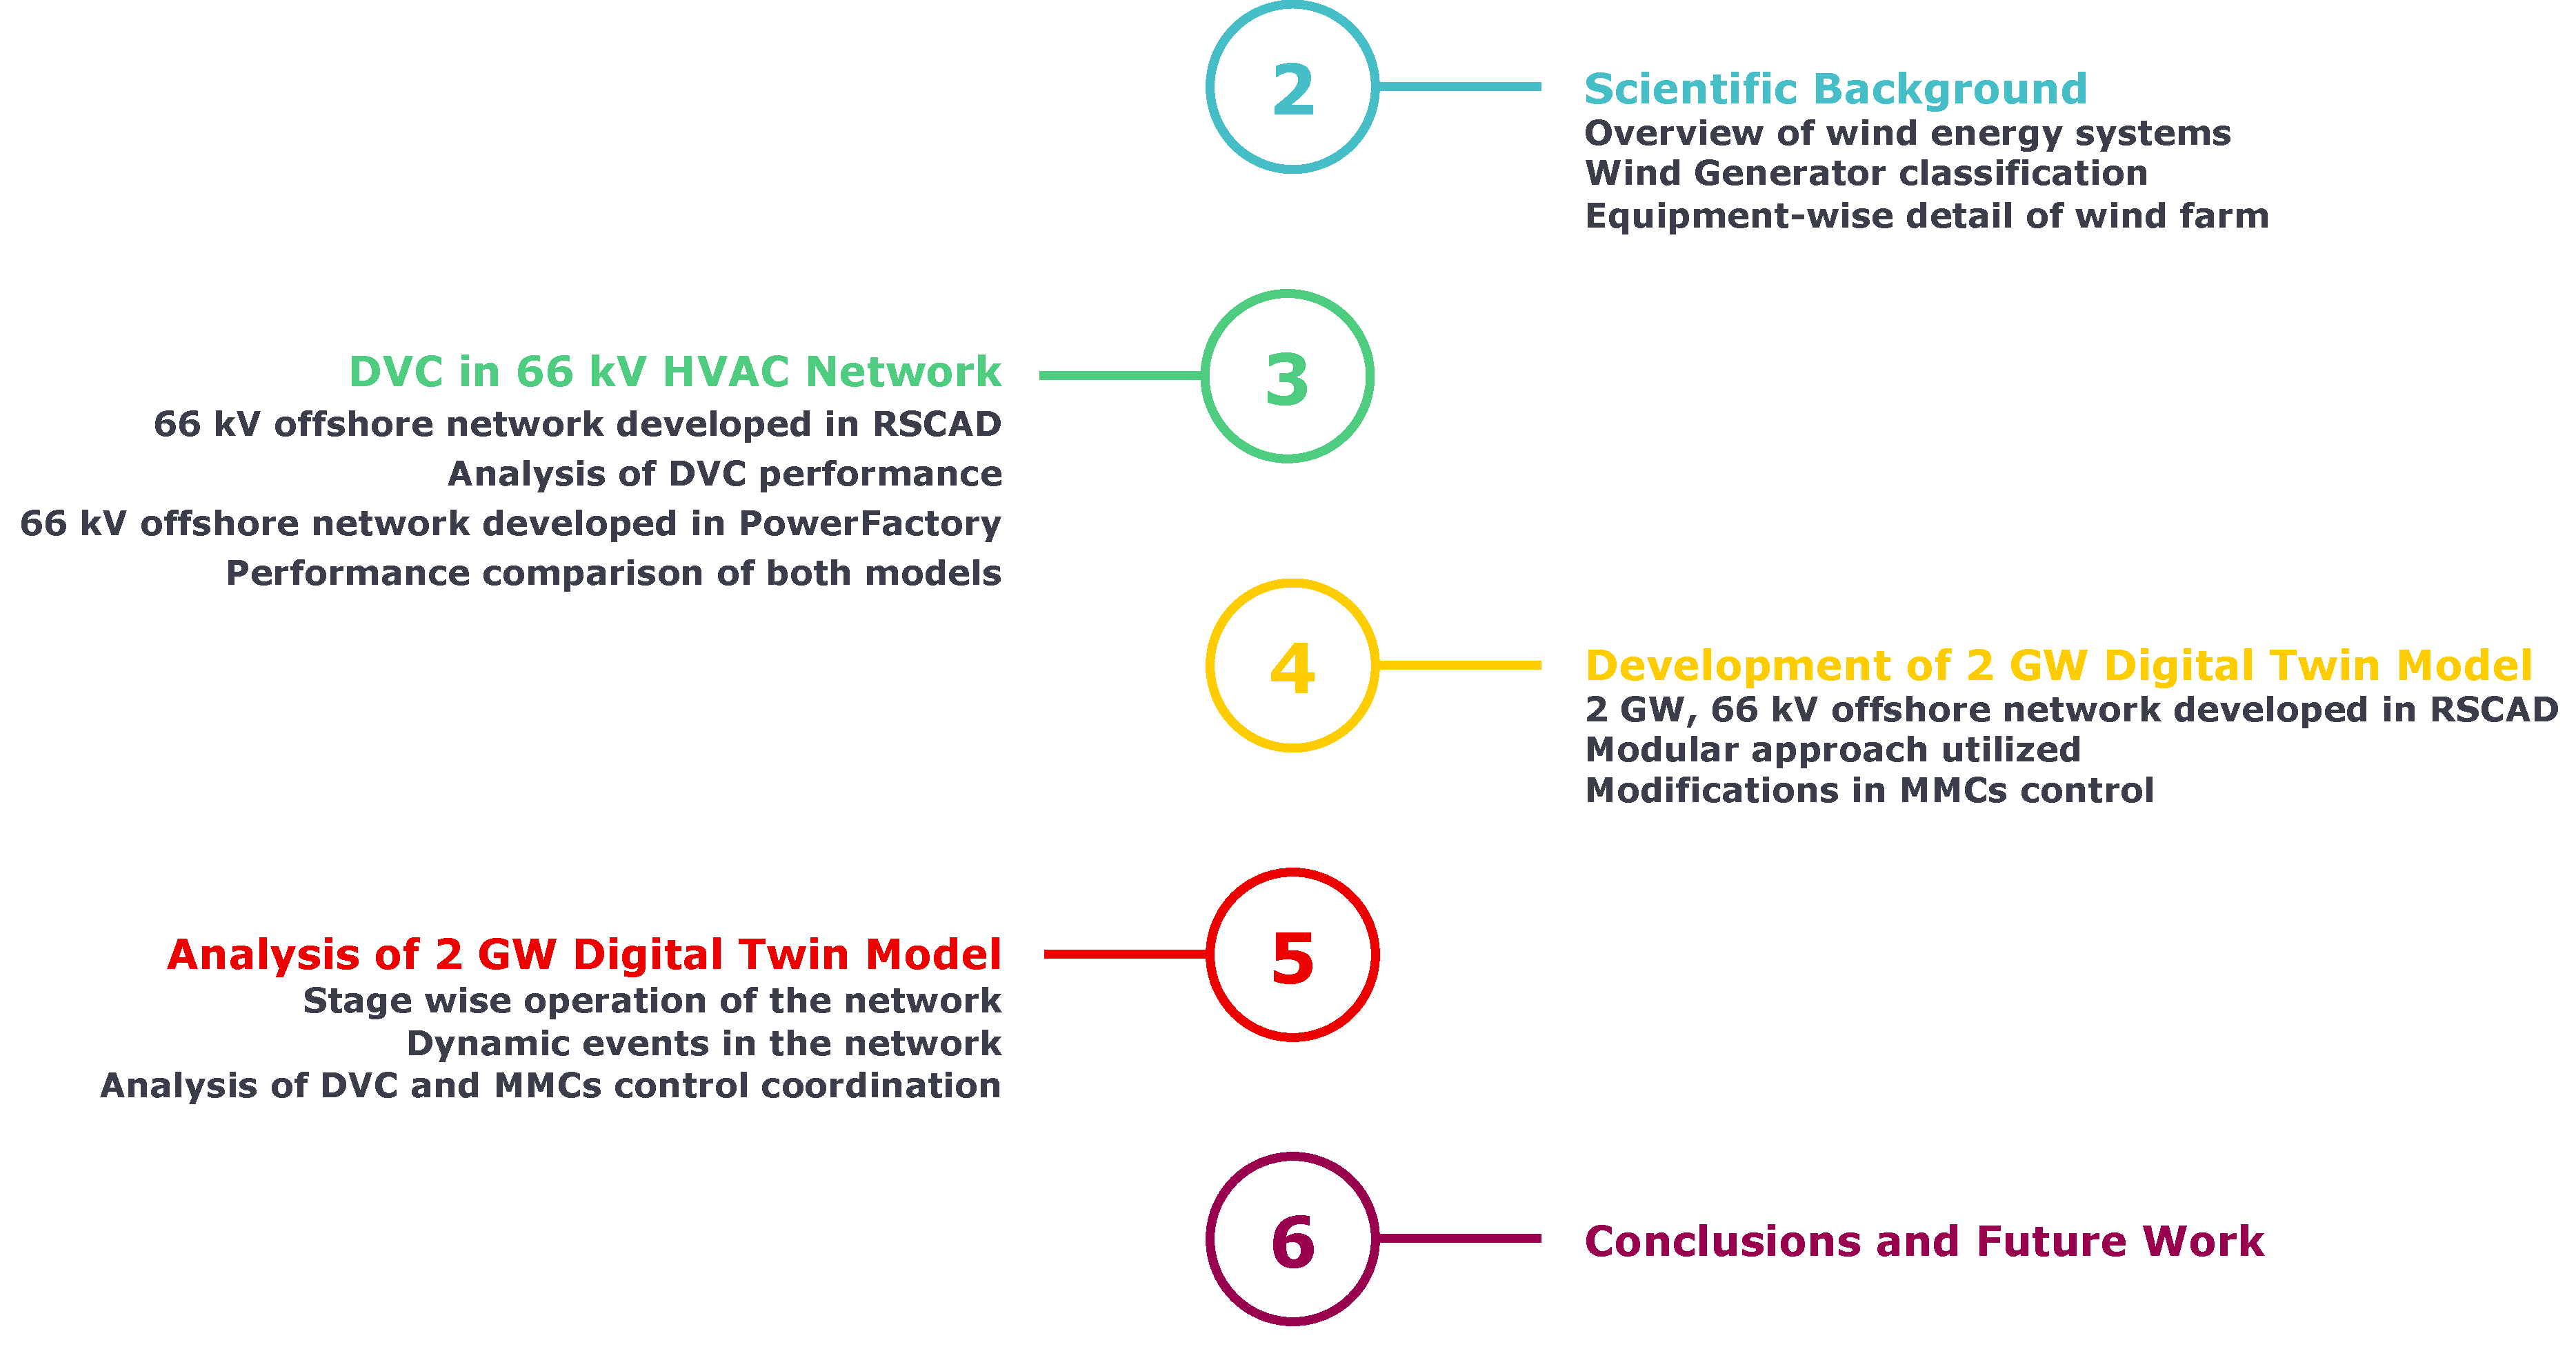
\includegraphics[height = 9.5cm,width =\textwidth]{Diagrams/Chapter_1/Thesis_flowchart.pdf}
    \caption{Work Flow of Thesis}
    \label{fig:Thesis_outline}
\end{figure}
